\documentclass[11pt,a4paper,twoside]{book}\usepackage[]{graphicx}\usepackage[]{color}
%% maxwidth is the original width if it is less than linewidth
%% otherwise use linewidth (to make sure the graphics do not exceed the margin)
\makeatletter
\def\maxwidth{ %
  \ifdim\Gin@nat@width>\linewidth
    \linewidth
  \else
    \Gin@nat@width
  \fi
}
\makeatother

\definecolor{fgcolor}{rgb}{0.345, 0.345, 0.345}
\newcommand{\hlnum}[1]{\textcolor[rgb]{0.686,0.059,0.569}{#1}}%
\newcommand{\hlstr}[1]{\textcolor[rgb]{0.192,0.494,0.8}{#1}}%
\newcommand{\hlcom}[1]{\textcolor[rgb]{0.678,0.584,0.686}{\textit{#1}}}%
\newcommand{\hlopt}[1]{\textcolor[rgb]{0,0,0}{#1}}%
\newcommand{\hlstd}[1]{\textcolor[rgb]{0.345,0.345,0.345}{#1}}%
\newcommand{\hlkwa}[1]{\textcolor[rgb]{0.161,0.373,0.58}{\textbf{#1}}}%
\newcommand{\hlkwb}[1]{\textcolor[rgb]{0.69,0.353,0.396}{#1}}%
\newcommand{\hlkwc}[1]{\textcolor[rgb]{0.333,0.667,0.333}{#1}}%
\newcommand{\hlkwd}[1]{\textcolor[rgb]{0.737,0.353,0.396}{\textbf{#1}}}%
\let\hlipl\hlkwb

\usepackage{framed}
\makeatletter
\newenvironment{kframe}{%
 \def\at@end@of@kframe{}%
 \ifinner\ifhmode%
  \def\at@end@of@kframe{\end{minipage}}%
  \begin{minipage}{\columnwidth}%
 \fi\fi%
 \def\FrameCommand##1{\hskip\@totalleftmargin \hskip-\fboxsep
 \colorbox{shadecolor}{##1}\hskip-\fboxsep
     % There is no \\@totalrightmargin, so:
     \hskip-\linewidth \hskip-\@totalleftmargin \hskip\columnwidth}%
 \MakeFramed {\advance\hsize-\width
   \@totalleftmargin\z@ \linewidth\hsize
   \@setminipage}}%
 {\par\unskip\endMakeFramed%
 \at@end@of@kframe}
\makeatother

\definecolor{shadecolor}{rgb}{.97, .97, .97}
\definecolor{messagecolor}{rgb}{0, 0, 0}
\definecolor{warningcolor}{rgb}{1, 0, 1}
\definecolor{errorcolor}{rgb}{1, 0, 0}
\newenvironment{knitrout}{}{} % an empty environment to be redefined in TeX

\usepackage{alltt}
% We load package by package and set package relevant parameters.
% Topics are summarized later
%%%%%%%%%%%%%%%%%%%%%%%%%%%%%%%%%%%%%%%%%%%%%%%%%%%%%%%%%%%%%%%%%%%%%%%%
% helping packages
\usepackage{ifthen}
\usepackage{calc}

\usepackage[T1]{fontenc}       % provides fonts having  accented characters 
\usepackage[latin1]{inputenc}  % allows the user to input accented characters directly from the keyboard

%%%%%%%%%%%%%%%%%%%%%%%%%%%%%%%%%%%%%%%%%%%%%%%%%%%%%%%%%%%%%%%%%%%%%%%%

\renewcommand{\baselinestretch}{1.2}
\renewcommand{\textfraction}{0}%0.2     % placement of figures
\renewcommand{\topfraction}{1}%.3
\renewcommand{\bottomfraction}{1}%.3
\renewcommand{\floatpagefraction}{1}%.3
\setcounter{bottomnumber}{3}%1

\textwidth6.3in
\textheight9.7in
\topmargin-45pt
\oddsidemargin-.15in
\evensidemargin.15in
\headsep30pt
\headheight15pt
%\footskip20pt


%%%%%%%%%%%%%%%%%%%%%%%%%%%%%%%%%%%%%%%%%%%%%%%%%%%%%%%%%%%%%%%%%%%%%%%%

\usepackage[dvipsnames]{xcolor}
\definecolor{fgcolor}{rgb}{0.345, 0.345, 0.345}
\definecolor{shadecolor}{rgb}{.97, .97, .97}
\definecolor{messagecolor}{rgb}{0, 0, 0}
\definecolor{warningcolor}{rgb}{1, 0, 1}
\definecolor{errorcolor}{rgb}{1, 0, 0}
\definecolor{DarkBlue}{rgb}{0,0,0.5451}
\definecolor{DarkGreen}{rgb}{0,0.39216,0}
\definecolor{LightYellow}{rgb}{1,1,.8}
\definecolor{orange}{rgb}{.9,0.3445,0}



%%%%%%%%%%%%%%%%%%%%%%%%%%%%%%%%%%%%%%%%%%%%%%%%%%%%%%%%%%%%%%%%%%%%%%%%
\usepackage{afterpage}
\usepackage{natbib}
\usepackage{upquote}

\usepackage[english]{babel}

%%%%%%%%%%%%%%%%%%%%%%%%%%%%%%%%%%%%%%%%%%%%%%%%%%%%%%%%%%%%%%%%%%%%%%%%%%%%%%%
%% maxwidth is the original width if it is less than linewidth
%% otherwise use linewidth (to make sure the graphics do not exceed the margin)
\makeatletter
\def\maxwidth{ %
  \ifdim\Gin@nat@width>\linewidth
    \linewidth
  \else
    \Gin@nat@width
  \fi
}
\makeatother

%%%%%%%%%%%%%%%%%%%%%%%%%%%%%%%%%%%%%%%%%%%%%%%%%%%%%%%%%%%%%%%%%%%%%%%%%%%%%%%%%%%%%%%%%%%%%%%%%%%%%%%%%%%%
% from fancyvrb
\usepackage{fancyhdr}
\usepackage{fancyvrb}
\DefineVerbatimEnvironment{Rcode}{Verbatim}{xleftmargin=2em,fontshape=sl,formatcom=\color{DarkGreen}}
\fvset{listparameters={\setlength{\topsep}{0pt}}}

%%%%%%%%%%%%%%%%%%%%%%%%%%%%%%%%%%%%%%%%%%%%%%%%%%%%%%%%%%%%%%%%%%%%%%%%%%%%%%%%%%%%%%%%%%%%%%%%%%%%%%%%%%%%%
\usepackage{float}
\usepackage{graphicx}
\usepackage[margin=2em,labelfont=bf]{caption}


%%%%%%%%%%%%%%%%%%%%%%%%%%%%%%%%%%%%%%%%%%%%%%%%%%%%%%%%%%%%%%%%%%%%%%%%
\usepackage[pdftex,plainpages=false,pdfpagelabels,pagebackref=true,colorlinks=true,pdfpagemode=UseOutlines]{hyperref}


%%%%%%%%%%%%%%%%%%%%%%%%%%%%%%%%%%%%%%%%%%%%%%%%%%%%%%%%%%%%%%%%%%%%%%%%
% now math stuff and other details...
\usepackage{amsmath,amsthm,amssymb}

\newtheorem{pro}{Property}[chapter]
\theoremstyle{definition}
\newtheorem{des}{Definition}[chapter]
\newtheorem{bsp}{Example}[chapter]
\newtheorem{rem}{Remark}[chapter]

\newcommand*\widebar[1]{%
  \vbox{%
    \hrule height 0.5pt%     % Line above with certain width
    \kern0.5ex%             % Distance between line and content
    \hbox{%
      \kern-0.1em%           % Distance between content and left side of box, negative values for lines shorter than content
      \ifmmode#1\else\ensuremath{#1}\fi%  % The content, typeset in dependence of mode
      \kern-0.1em%      % Distance between content and left side of box, negative values for lines shorter than content
    }% end of hbox
  }% end of vbox
}
\def\ds{\displaystyle}

\newcommand{\rr}[1]{{\ttfamily\slshape\color{DarkGreen} #1}}

\makeatletter


% clever trick to circumvent potential redefines after loading packages:
% \providecommand{\something}{}  % if it does not exist, it creates it.
%      has same syntax as \newcommand
% \renewcommand{\something}{....}
% TUGboat 29(2)


\makeatletter
%umdefinierung exisitierender befehle
\let\oldH\H
\let\oldL\L
\let\oldO\H
\let\oldS\S
\let\olda\a
\let\oldb\b
\let\oldc\c
\let\oldd\d
\let\oldk\k
\let\oldv\v
\let\oldl\l
\let\oldt\t
\let\oldu\u
\let\oldIJ\IJ
\let\oldP\P
\let\P\relax
\let\oldnorm\|

%\DefineVerbatimEnvironment{CodeInput}{Verbatim}{fontshape=sl}
%\DefineVerbatimEnvironment{CodeOutput}{Verbatim}{}

% some classical environments, up-right, with chapter numbering.
\theoremstyle{definition}
\newtheorem{definition}{Definition}[chapter]
\newtheorem{example}{Example}[chapter]
\newtheorem{remark}{Remark}[chapter]
\newtheorem{theorem}{Theorem}[chapter]



\renewcommand{\|}{|\!|}         % closer norm
\newcommand{\T}{{}^{\top}}
\newcommand\code[1]{{\tt#1}}



\newcounter{algo}
\newenvironment{algorithm}{%
  \begin{list}{
      (\arabic{algo})
    }{
      \usecounter{algo}
    }%
}{
  \end{list}
}

% some text abbreviation
\newcommand{\GLS}{\text{GLS}}
\newcommand{\RR}{\text{RR}}
\newcommand{\OR}{\text{OR}}
\newcommand{\WLS}{\text{WLS}}
\newcommand{\MLE}{\text{MLE}}
\newcommand{\OLS}{\text{OLS}}
\newcommand{\MAE}{\text{MAE}}
\newcommand{\MAD}{\text{MAD}}
\newcommand{\RMSE}{\text{RMSE}}

\newcommand{\ii}{\text{\i}}

\newcommand{\Bin}{\cB\mathit{\!i\!n}}
\newcommand{\Beta}{\cB\mathit{\!e\!t\!a}}
\newcommand{\Pois}{\cP\mathit{\!o\!i\!s\!s\!o\!n}}
\newcommand{\Exp}{\cE\mathit{\!x\!p}}


\DeclareMathOperator*{\argmin}{argmin}
\DeclareMathOperator*{\argmax}{argmax}
\DeclareMathOperator{\diag}{diag}
\DeclareMathOperator{\diam}{diam}
\DeclareMathOperator{\card}{card}
\DeclareMathOperator{\cov}{Cov}                   
\DeclareMathOperator{\corr}{Corr}                 
\DeclareMathOperator{\var}{Var}                   
\DeclareMathOperator{\trace}{tr}                  
\DeclareMathOperator{\E}{E}                       
\DeclareMathOperator{\P}{P}                       
\DeclareMathOperator{\pred}{p}
\DeclareMathOperator{\vect}{vec}                  
\DeclareMathOperator{\vech}{vech}                 
\DeclareMathOperator{\rank}{rank}                 
\DeclareMathOperator{\e}{e}                       
%\DeclareMathOperator{\cv}{CV}                     
\DeclareMathOperator{\GCV}{GCV}                     
\DeclareMathOperator{\CV}{CV}                     
\DeclareMathOperator{\BLUP}{BLUP}                 
\DeclareMathOperator{\MSE}{MSE}                   
\DeclareMathOperator{\MS}{MS}                   
\DeclareMathOperator{\df}{df}                   
\DeclareMathOperator{\bias}{bias}                   
\DeclareMathOperator{\eig}{eig}                   
\DeclareMathOperator{\Prec}{Prec}
\DeclareMathOperator{\mode}{mode}
\renewcommand{\SS}{\text{SS}}
\renewcommand{\d}{\mathsf{\,d}}

\def\arctanh{\qopname\relax o{arctanh}}  % as in amsopn
\newcommand{\bigo}{\cO}
\newcommand{\lito}{\text{\scriptsize{$\cO$}}}
\newcommand{\cdfPhi}{\itPhi}
\newcommand{\ml}{_\text{ML}}

\newcommand*{\stack@relbin}[3][]{%
  \mathop{#3}\limits
  \toks@{#1}%
  \edef\reserved@a{\the\toks@}%
  \ifx\reserved@a\@empty\else_{#1}\fi
  \toks@{#2}%
  \edef\reserved@a{\the\toks@}%
  \ifx\reserved@a\@empty\else^{#2}\fi
  \egroup
}%
\renewcommand*{\stackrel}{\mathrel\bgroup\stack@relbin}
\newcommand*{\stackbin}{\mathbin\bgroup\stack@relbin}
\newcommand{\simiid}{\stackrel[]{\text{iid}}{\sim}}

% Kalligraphischer Schriftsatz
\newcommand{\cA}{{\cal{A}}}
\newcommand{\cB}{{\cal{B}}} 
\newcommand{\cC}{{\cal{C}}}
\newcommand{\cD}{{\cal{D}}} 
\newcommand{\cE}{{\cal{E}}}
\newcommand{\cF}{{\cal{F}}}
\newcommand{\cG}{{\cal{G}}}
\newcommand{\cH}{{\cal{H}}}
\newcommand{\cI}{{\cal{I}}}
\newcommand{\cJ}{{\cal{J}}}
\newcommand{\cK}{{\cal{K}}}
\newcommand{\cL}{{\cal{L}}}
\newcommand{\cM}{{\cal{M}}} 
\newcommand{\cN}{{\cal{N}}}
\newcommand{\cO}{{\cal{O}}} 
\newcommand{\cP}{{\cal{P}}}
\newcommand{\cQ}{{\cal{Q}}} 
\newcommand{\cR}{{\cal{R}}} 
\newcommand{\cS}{{\cal{S}}} 
\newcommand{\cT}{{\cal{T}}}
\newcommand{\cU}{{\cal{U}}}
\newcommand{\cV}{{\cal{V}}}
\newcommand{\cW}{{\cal{W}}}
\newcommand{\cX}{{\cal{X}}} 
\newcommand{\cY}{{\cal{Y}}}
\newcommand{\cZ}{{\cal{Z}}} 


\newcommand{\IA}{{\mathbb{A}}}
\newcommand{\IB}{{\mathbb{B}}}
\newcommand{\IC}{{\mathbb{C}}}
\newcommand{\ID}{{\mathbb{D}}}
\newcommand{\IE}{{\mathbb{E}}}
\newcommand{\IF}{{\mathbb{F}}}
\newcommand{\IG}{{\mathbb{G}}}
\newcommand{\IH}{{\mathbb{H}}}
\newcommand{\II}{{\mathbb{I}}}
%\newcommand{\IJ}{{\mathbb{J}}}
\newcommand{\IK}{{\mathbb{K}}}
\newcommand{\IL}{{\mathbb{L}}}
\newcommand{\IM}{{\mathbb{M}}}
\newcommand{\IN}{{\mathbb{N}}}
\newcommand{\IO}{{\mathbb{O}}}
\newcommand{\IP}{{\mathbb{P}}}
\newcommand{\IQ}{{\mathbb{Q}}}
\newcommand{\IR}{{\mathbb{R}}}
\newcommand{\IS}{{\mathbb{S}}}
\newcommand{\IT}{{\mathbb{T}}}
\newcommand{\IU}{{\mathbb{U}}}
\newcommand{\IV}{{\mathbb{V}}}
\newcommand{\IW}{{\mathbb{W}}}
\newcommand{\IX}{{\mathbb{X}}}
\newcommand{\IY}{{\mathbb{Y}}}
\newcommand{\IZ}{{\mathbb{Z}}}


% fette griechische kleinbuchstaben
\newcommand{\balpha}{{\boldsymbol{\alpha}}}
\newcommand{\bbeta}{{\boldsymbol{\beta}}}
\newcommand{\bgamma}{{\boldsymbol{\gamma}}}
\newcommand{\bdelta}{{\boldsymbol{\delta}}}
\newcommand{\blambda}{{\boldsymbol{\lambda}}}
\newcommand{\bepsilon}{{\boldsymbol{\epsilon}}}
\newcommand{\bvarepsilon}{{\boldsymbol{\varepsilon}}}
\newcommand{\bzeta}{{\boldsymbol{\zeta}}}
\newcommand{\bfeta}{{\boldsymbol{\eta}}}  %  <----- exception !
\newcommand{\btheta}{{\boldsymbol{\theta}}{}}
\newcommand{\bvartheta}{{\boldsymbol{\vartheta}}}
\newcommand{\biota}{{\boldsymbol{\iota}}}
\newcommand{\bkappa}{{\boldsymbol{\kappa}}}
\newcommand{\bmu}{{\boldsymbol{\mu}}}
\newcommand{\bnu}{{\boldsymbol{\nu}}}
\newcommand{\bxi}{{\boldsymbol{\xi}}}
\newcommand{\bpi}{{\boldsymbol{\pi}}}
\newcommand{\bvarpi}{{\boldsymbol{\varpi}}}
\newcommand{\brho}{{\boldsymbol{\rho}}}
\newcommand{\bvarrhoi}{{\boldsymbol{\varrho}}}
\newcommand{\bsigma}{{\boldsymbol{\sigma}}}
\newcommand{\bvarsigma}{{\boldsymbol{\varsigma}}}
\newcommand{\btau}{{\boldsymbol{\tau}}}
\newcommand{\bvartau}{{\boldsymbol{\vartau}}}
\newcommand{\bupsilon}{{\boldsymbol{\upsilon}}}
\newcommand{\bphi}{{\boldsymbol{\phi}}}
\newcommand{\bvarphi}{{\boldsymbol{\varphi}}}
\newcommand{\bchi}{{\boldsymbol{\chi}}}
\newcommand{\bpsi}{{\boldsymbol{\psi}}}
\newcommand{\bomega}{{\boldsymbol{\omega}}}


% fette griechische grossbuchstaben
\newcommand{\bGamma}{{\boldsymbol{\Gamma}}}
\newcommand{\bDelta}{{\boldsymbol{\Delta}}}
\newcommand{\bTheta}{{\boldsymbol{\Theta}}}
\newcommand{\bLambda}{{\boldsymbol{\Lambda}}{}}
\newcommand{\bXi}{{\boldsymbol{\Xi}}}
\newcommand{\bPi}{{\boldsymbol{\Pi}}}
\newcommand{\bSigma}{{\boldsymbol{\Sigma}}{}}
\newcommand{\bUpsilon}{{\boldsymbol{\Upsilon}}{}}
\newcommand{\bPhi}{{\boldsymbol{\Phi}}}
\newcommand{\bPsi}{{\boldsymbol{\Psi}}}
\newcommand{\bOmega}{{\boldsymbol{\Omega}}}

% italics griechische grossbuchstaben
\newcommand{\itGamma}{{\mathit{\Gamma}}}
\newcommand{\itDelta}{{\mathit{\Delta}}}
\newcommand{\itTheta}{{\mathit{\Theta}}}
\newcommand{\itLambda}{{\mathit{\Lambda}}}
\newcommand{\itXi}{{\mathit{\Xi}}}
\newcommand{\itPi}{{\mathit{\Pi}}}
\newcommand{\itSigma}{{\mathit{\Sigma}}}
\newcommand{\itUpsilon}{{\mathit{\Upsilon}}}
\newcommand{\itPhi}{{\mathit{\Phi}}}
\newcommand{\itPsi}{{\mathit{\Psi}}}
\newcommand{\itOmega}{{\mathit{\Omega}}}



\newcommand{\A}{{\mathbf{A}}}
\newcommand{\B}{{\mathbf{B}}}
\newcommand{\C}{{\mathbf{C}}}
\newcommand{\D}{{\mathbf{D}}}
\newcommand{\bfE}{{\mathbf{E}}}    % \E: expectation
\newcommand{\F}{{\mathbf{F}}}
\newcommand{\G}{{\mathbf{G}}}
\renewcommand{\H}{{\mathbf{H}}}
\newcommand{\I}{{\mathbf{I}}}
\newcommand{\J}{{\mathbf{J}}}
\newcommand{\K}{{\mathbf{K}}}
\renewcommand{\L}{{\mathbf{L}}}
\newcommand{\bfM}{{\mathbf{M}}}
\newcommand{\N}{{\mathbf{N}}}
\renewcommand{\O}{{\mathbf{O}}}
\newcommand{\bfP}{{\mathbf{P}}}  % \P : probability
\newcommand{\Q}{{\mathbf{Q}}}
\newcommand{\bfR}{{\mathbf{R}}}
\renewcommand{\S}{{\mathbf{S}}}
\newcommand{\bfT}{{\mathbf{T}}} % \T transpose
\newcommand{\U}{{\mathbf{U}}}
\newcommand{\V}{{\mathbf{V}}}
\newcommand{\W}{{\mathbf{W}}}
\newcommand{\X}{{\mathbf{X}}}
\newcommand{\Y}{{\mathbf{Y}}}
\newcommand{\Z}{{\mathbf{Z}}}


\newcommand{\0}{{\mathbf{0}}}
\newcommand{\1}{{\mathbf{1}}}
\newcommand{\2}{{\mathbf{2}}}
\newcommand{\3}{{\mathbf{3}}}
\newcommand{\4}{{\mathbf{4}}}
\newcommand{\5}{{\mathbf{5}}}
\newcommand{\6}{{\mathbf{6}}}
\newcommand{\7}{{\mathbf{7}}}
\newcommand{\8}{{\mathbf{8}}}
\newcommand{\9}{{\mathbf{9}}}

\renewcommand{\a}{{\textbf{\textit{a}}}}
\renewcommand{\b}{{\textbf{\textit{b}}}}
\renewcommand{\c}{{\textbf{\textit{c}}}}
\newcommand{\bfd}{{\textbf{\textit{d}}}}  % \d  'dx'
\newcommand{\bfe}{{\textbf{\textit{e}}}}  % \e  l'exponentiel
\newcommand{\f}{{\textbf{\textit{f}}}}
\newcommand{\g}{{\textbf{\textit{g}}}}
\newcommand{\h}{{\textbf{\textit{h}}}}
\newcommand{\bfi}{{\textbf{\textit{i}}}}%\i  complex i, sans 'dot'
\newcommand{\bfj}{{\textbf{\textit{j}}}}
\renewcommand{\l}{{\textbf{\textit{l}}}}
\renewcommand{\k}{{\textbf{\textit{k}}}}
\newcommand{\m}{{\textbf{\textit{m}}}}
\newcommand{\bfn}{{\textbf{\textit{n}}}}
\newcommand{\bfo}{{\textbf{\textit{o}}}}
\newcommand{\p}{{\textbf{\textit{p}}}}
\newcommand{\q}{{\textbf{\textit{q}}}}
\renewcommand{\r}{{\textbf{\textit{r}}}}
\newcommand{\s}{{\textbf{\textit{s}}}}
\renewcommand{\t}{{\textbf{\textit{t}}}}
\newcommand{\bfu}{{\textbf{\textit{u}}}} %\u used in references
\renewcommand{\v}{{\textbf{\textit{v}}}}
\newcommand{\w}{{\textbf{\textit{w}}}}
\newcommand{\x}{{\textbf{\textit{x}}}}
\newcommand{\y}{{\textbf{\textit{y}}}}
\newcommand{\z}{{\textbf{\textit{z}}}}




\ifcsname hlkwd\endcsname%    ... command '#1' exists ...%
\else%  ... command '#1' does not exist ...%

\def\maxwidth{ %
  \ifdim\Gin@nat@width>\linewidth
    \linewidth
  \else
    \Gin@nat@width
  \fi
}

\definecolor{fgcolor}{rgb}{0.345, 0.345, 0.345}
\newcommand{\hlnum}[1]{\textcolor[rgb]{0.686,0.059,0.569}{#1}}%
\newcommand{\hlstr}[1]{\textcolor[rgb]{0.192,0.494,0.8}{#1}}%
\newcommand{\hlcom}[1]{\textcolor[rgb]{0.678,0.584,0.686}{\textit{#1}}}%
\newcommand{\hlopt}[1]{\textcolor[rgb]{0,0,0}{#1}}%
\newcommand{\hlstd}[1]{\textcolor[rgb]{0.345,0.345,0.345}{#1}}%
\newcommand{\hlkwa}[1]{\textcolor[rgb]{0.161,0.373,0.58}{\textbf{#1}}}%
\newcommand{\hlkwb}[1]{\textcolor[rgb]{0.69,0.353,0.396}{#1}}%
\newcommand{\hlkwc}[1]{\textcolor[rgb]{0.333,0.667,0.333}{#1}}%
\newcommand{\hlkwd}[1]{\textcolor[rgb]{0.737,0.353,0.396}{\textbf{#1}}}%

\usepackage{framed}
\newenvironment{kframe}{%
 \def\at@end@of@kframe{}%
 \ifinner\ifhmode%
  \def\at@end@of@kframe{\end{minipage}}%
  \begin{minipage}{\columnwidth}%
 \fi\fi%
 \def\FrameCommand##1{\hskip\@totalleftmargin \hskip-\fboxsep
 \colorbox{shadecolor}{##1}\hskip-\fboxsep
     % There is no \\@totalrightmargin, so:
     \hskip-\linewidth \hskip-\@totalleftmargin \hskip\columnwidth}%
 \MakeFramed {\advance\hsize-\width
   \@totalleftmargin\z@ \linewidth\hsize
   \@setminipage}}%
 {\par\unskip\endMakeFramed%
 \at@end@of@kframe}
\renewenvironment{kframe}{%
 \def\at@end@of@kframe{}%
 \ifinner\ifhmode%
  \def\at@end@of@kframe{\end{minipage}}%
  \begin{minipage}{\columnwidth}%
 \fi\fi%
 \def\FrameCommand##1{\hskip\@totalleftmargin \hskip-0\fboxsep
 \colorbox{shadecolor}{##1}\hskip-0\fboxsep
     % There is no \\@totalrightmargin, so:
     \hskip-\linewidth \hskip-\@totalleftmargin \hskip\columnwidth}%
 \MakeFramed {\advance\hsize-\width
   \@totalleftmargin\z@ \linewidth\hsize
   \@setminipage}}%
 {\par\unskip\endMakeFramed%
 \at@end@of@kframe}


\definecolor{shadecolor}{rgb}{.97, .97, .97}
\definecolor{messagecolor}{rgb}{0, 0, 0}
\definecolor{warningcolor}{rgb}{1, 0, 1}
\definecolor{errorcolor}{rgb}{1, 0, 0}
%\newenvironment{knitrout}{}{} % an empty environment to be redefined in TeX
\newenvironment{knitrout}{\setlength{\topsep}{0mm}\setlength{\fboxsep}{4mm}}{} 

\usepackage{alltt}
\IfFileExists{upquote.sty}{\usepackage{upquote}}{}

  \fi%

\makeatother
   % packages, layout and standard macros


\usepackage{verbatim}
\usepackage{tikz}
\usetikzlibrary{trees}
\IfFileExists{upquote.sty}{\usepackage{upquote}}{}
\begin{document}
\renewcommand\familydefault{\sfdefault} 
\pagenumbering{Alph}


\thispagestyle{empty}
\renewcommand{\baselinestretch}{1.5}\normalfont
\begin{center}
\setlength{\parindent}{0cm}
\bf\Large% 
Publication Bias in the Cochrane Database of Systematic Review \\
Application of tests and adjustment methods for publication bias in meta-analyses
\normalfont



\hrulefill

\vspace*{4cm}

\large
Master Thesis in Biostatistics (STA495) % or choose the next one
% Master Thesis in Mathematics (MAT491) 
\vspace*{12mm}

by

\vspace*{12mm}

Giuachin Kreiliger\\
\small 12123832\\
\normalfont
\vspace*{4cm}

supervised by

\vspace*{1cm}

Dr. Simon Schwab\\
Prof. Leonhard Held

\vfill

Zurich, month year
\end{center}
\renewcommand\familydefault{\rmdefault}%
\renewcommand{\baselinestretch}{1.0}\rm 
\setcounter{page}{0}
\newpage
\vspace*{12cm}~\thispagestyle{empty}\pagenumbering{Roman}
\newpage





\graphicspath{{./figure/}}
\DeclareGraphicsExtensions{.pdf,.png}
\setcounter{tocdepth}{1}



\thispagestyle{empty}
\begin{center}
  \vspace*{6cm}{\bfseries\Huge
  $p$-values:\\[5mm] their use, abuse and proper use \\[5mm]
  illustrated with seven facets 
  }
  \vfill
  \rm

  \LARGE
  M\"axli Musterli\\[12mm]
  
  \normalsize
  Version \today
\end{center}
\newpage
\thispagestyle{empty}~
\newpage
\pagenumbering{roman}

\thispagestyle{plain}\markboth{Contents}{Contents}
\tableofcontents
\setkeys{Gin}{width=.8\textwidth}

\chapter*{Preface}
\addtocontents{toc}{\protect \vspace*{13.mm}}
\addcontentsline{toc}{chapter}{\bfseries{Preface}}
\thispagestyle{plain}\markboth{Preface}{Preface}

Howdy!

\bigskip

\begin{flushright}
  Max Muster\\
  June 2018
\end{flushright}

\addtocontents{toc}{\protect \vspace*{10mm}}

\cleardoublepage
\pagenumbering{arabic}


%%%%%%%%%%%%%%%%%%%%%%%%%%%%%%%%%%%%%%%%%%%%%%%%%%%%%%%%%%%%%%%%%%%%%%


% LaTeX file for Chapter 01



\chapter{Introduction}

In science, there is not only a need for accumulation of knowledge, but also for concentration. For the same reason as statistical analysis is performed on single experiments, it can also be used for results of multiple experiments or studies: to simplify and summarize the data at hand to a degree that is understandable for humans. The latter procedure goes usually under the term of meta-analysis. Meta analyses are used to summarize results and evidence over multiple studies when they are considered to be similar enough.

\vspace{0mm}
In the face of the large amount of research that is done in some fields of empirical science, meta-analysis becomes increasingly important, for looking at all evidence would simply take very long for one person. Meta-analysises are often part of a systematic review, an effort of experts of a field to provide an overlook over the evidence. In the course of a review, all literature and data with respect to a scientific question is collected and a meta-analysis is operated at the end to summarize the findings.

\vspace{0mm}
In the case of clinical science, systematic reviews and meta-analyses do not only benefit scientists but also patients and clinicians, for both are provided with up-to-date summaries of current evidence with respect to a certain treatment. Therefore, meta-analysis is at the core of what is called evidence-based medicine. 

\vspace{0mm}
However, there are problems that potentially limit the validity of meta-analysis; studies at hand can be biased or heterogeneity between study results can be large and the number of studies small. The importance and the issues of meta-analysis are the reasons why they have been chosen as one general topic of the masters thesis. One particular problem will furthermore be investigated in more detail: reporting bias and meta-analysis. Not only will the methods to deal with issues as reporting bias be discussed, but also will they be applied on a dataset of systematic reviews that can be used for meta-analysis. So at the end of the report, the reader will not only have an impression of the technical issues caused by reporting bias, but also of the abundance and extent of it in the dataset. Since the dataset is very large and of good quality, results might be again be generalizable to some extent to reporting bias in clinical science in general.


\subsection{Cochrane and the Cochrane Database of Systematic Reviews}
The Cochrane Organization has specialized on systematic reviews in clinical science. It publishes and maintains a library with a large number of systematic reviews that are available in some countries to the public.

\vspace{0mm}
The data analyzed in this thesis stems completely from the Cochrane Library of systematic Reviews (cite). The reviews are arguably of good quality, since the authors are following elaborated guidelines, and there are control-mechanisms within the organisation that should prohibit conflicts of interests. This might further improve the validity and precision of findings and conclusions that have been made based on this data. 




%%%%%%%%%%%%%%%%%%%%%%%%%%%%%%%%%%%%%%%%%%%%%%%%%%%%%%%%%%%%%%%%%%%%%%


% LaTeX file for Chapter 02











\chapter{The Cochrane Dataset} 

\subsection{Structure and Content}
The dataset consists of 5016 systematic reviews from the Cochrane Library with 52995 studies.
Each study provides data of (multiple) comparisons of clinical interventions. 
% It can not be ruled out that some comparisons are retrospective, e.g. from observational studies. 
In Table \ref{barbiturate.row}, two comparisons from a systematic review about effects of barbiturates are shown as they are given in the dataset. As can be seen, the comparison is further specified by the variables in the columns. One row of the dataset is one comparison.

% latex table generated in R 3.5.1 by xtable 1.8-3 package
% Thu Mar 21 11:15:04 2019
\begin{table}[ht]
\centering
\begingroup\scriptsize
\begin{tabular}{lllrrrr}
  \hline
Study & Comparison\_type & Outcome & Events & Total & Events\_c & Total\_c \\ 
  \hline
Bohn 1989 & Barbiturate vs no barbiturate & Death at the end of follow-up &  11 &  41 &  11 &  41 \\ 
  Ward 1985 & Barbiturate vs no barbiturate & Death at the end of follow-up &  14 &  27 &  13 &  26 \\ 
   \hline
\end{tabular}
\endgroup
\caption{Example of two comparisons as given in the dataset. Events denotes the count of events in the treatment group while Events c the count of events in the group compared to. Further descriptive variables have been ommitted} 
\label{barbiturate.row}
\end{table}


A complete listing of the variables is given in Table \ref{variable}. They can roughly be separated into variables that specify the review in which the comparison is contained and variables that specify the comparison itself (separated by a horizontal line in Table \ref{variable}).

\begin{table}[ht]
  \begin{center}
    \begin{tabular}{l l}
      \textbf{Variable} & \textbf{Description}\\
      \hline
      \textbf{File name} & The name of the file from which the review data has been . \\&gathered. This file corresponds to a file available in the. \\& Cochrane library\\
      \textbf{doi} & Digital object identifier. A unique id of the review such that  \\ &the full text of the review can be found on the web.\\
      \textbf{File index} & Internal index of the file in the Cochrane library.\\
      \textbf{File version} & Denotes the version of the review, since the reviews are \\ &occasionally updated.\\
      %\multicolumn{2}{c}{textbf{Study level variables}}\\ 
      \hline
      \textbf{Comparison type} & Specification of the interventions compared in the study\\
      \textbf{Outcome} & Specification by which outcome the interventions are compared\\
      \textbf{Subgroup} & Potentially indication of affiliation to subgroups\\
      \textbf{Study name} & Name of the study to which the comparison belongs\\
      \textbf{Study publication year} & Year in which the study was published\\
      \textbf{Outcome measure} & Indication of the quantification method of the effect \\ &(of one intervention compared to the other).\\
      \textbf{Effect} & Measure of the effect given in the quantity denoted by \\ &``outcome measure''.\\
      \textbf{Events (1/2)} & The counts of patients with an outcome \textit{if}\\ & measurement/outcome is binary or dichotomous \\ &2 (1 for treatment group and 2 for control group).\\
      \textbf{Total (1/2)} & Number of patients in groups.\\
      \textbf{Mean (1/2)} & Mean of patient measurements \textit{if} outcome is continuous.\\
      \textbf{Standard deviation (1/2)} & Standard deviation of mean \textit{if} \\ &outcome is continuous.
    \end{tabular}
  \caption{Dataset variable descriptions}
  \label{variable}
  \end{center}
\end{table}

The structure of a hypothetical review is shown in Figure \ref{review}. 
% Comparisons of a review can consecutively be subdivided into different comparison types, different outcome measures and different subgroups. 
The comparison type variable specifies what is compared, the outcome variable how it is compared, and the subgroup variable indicates if the comparison belongs to a certain subgroup. If desired, Figure \ref{review} can be compared to Table \ref{barbiturates} where an examplary review is listed.

\begin{figure}
\tikzstyle{every node}=[draw=black,thick,anchor=west]
\tikzstyle{selected}=[draw=red,fill=red!30]
\tikzstyle{optional}=[dashed,fill=gray!50]
\begin{tikzpicture}
[grow = right, anchor = west, 
  growth parent anchor=east, % added code
  parent anchor=east]
  \node {Review} [edge from parent fork right]
    child { node {Comparison type 2}
      child { node {Outcome 2}}
      child { node {Outcome 1}
        child { node {Subgroup 2}}
        child { node {Subgroup 1}}}
    }
    child [missing] {}		
    child { node {Comparison type 1  }};
\end{tikzpicture}
\caption{Structure of a hypothetical review with two different comparisons.}
\label{review.structure}
\end{figure}



% \vspace{0mm}
% Lets consider the previously mentioned barbiturate and head injury review. The aim was to ``assess the effects of barbiturates in reducing mortality, disability and raised ICP (intra-cranial pressure) in people with acute traumatic brain injury'' as well as to ``quantify any side effects resulting from the use of barbiturates''. The medical background is that one knew that barbiturates could cause relief in intra-cranial pressure, but also reduce cerebral blood flow. Because one effect is thought to be beneficial for persons with severe head injuries while the other isn't, the authors of the review wanted to find out if there is a net benefit of barbiturates.
% 
% \vspace{0mm}
% The review comprises five studies in total. Three of them compared barbiturate to placebo, one compared barbiturate to Mannitol and one Pentobarbital to Thiopental, which would be the comparison/research subject to speak in the previously introduced notions. 
% 
% \vspace{0mm}
% All the studies convey multiple information to the review. As an example, that could be death or death \textit{and} severe disability at follow up as an outcome. Again, the study can be further split up in different subgroups, here for example in a group with - and without haematoma. 
% 
% \vspace{0mm}
% The complete listing of outcomes is in table \ref{barbiturates}. The table also gives an illustration of the variety of data that can be included in a review. We have for example continuous and binary outcome data, that again is divided into a variety of different things that have been measured. Often, additionally to the main study result, also adverse effects are for example included which are in this case separate outcomes and possibly subgroups.


% latex table generated in R 3.5.1 by xtable 1.8-3 package
% Thu Mar 21 11:15:04 2019
\begin{table}[ht]
\centering
\begingroup\footnotesize
\begin{tabular}{lll}
  \hline
Study & Comparison & Outcome \\ 
  \hline
Bohn 1989 & Barbiturate vs no barbiturate & Death at the end of follow-up \\ 
  Bohn 1989 & Barbiturate vs no barbiturate & Death or severe disability at the end of follow-up \\ 
  Eisenberg 1988 & Barbiturate vs no barbiturate & Death at the end of follow-up \\ 
  Eisenberg 1988 & Barbiturate vs no barbiturate & Uncontrolled ICP during treatment \\ 
  Eisenberg 1988 & Barbiturate vs no barbiturate & Hypotension during treatment \\ 
  Perez-Barcena 2008 & Pentobarbital vs Thiopental & Death at the end of follow-up (6 months) \\ 
  Perez-Barcena 2008 & Pentobarbital vs Thiopental & Death or severe disability at the end of follow-up (6 months) \\ 
  Perez-Barcena 2008 & Pentobarbital vs Thiopental & Uncontrolled ICP during treatment \\ 
  Perez-Barcena 2008 & Pentobarbital vs Thiopental & Hypotension during treatment \\ 
  Schwartz 1984 & Barbiturate vs Mannitol & Death at the end of follow-up (1 year) \\ 
  Schwartz 1984 & Barbiturate vs Mannitol & Death at the end of follow-up (1 year) \\ 
  Schwartz 1984 & Barbiturate vs Mannitol & Uncontrolled ICP during treatment \\ 
  Ward 1985 & Barbiturate vs no barbiturate & Death at the end of follow-up \\ 
  Ward 1985 & Barbiturate vs no barbiturate & Death or severe disability at the end of follow-up \\ 
  Ward 1985 & Barbiturate vs no barbiturate & Mean ICP during treatment \\ 
  Ward 1985 & Barbiturate vs no barbiturate & Mean arterial pressure during treatment \\ 
  Ward 1985 & Barbiturate vs no barbiturate & Hypotension during treatment \\ 
  Ward 1985 & Barbiturate vs no barbiturate & Mean body temperature during treatment \\ 
   \hline
\end{tabular}
\endgroup
\caption{Barbiturate and head injury review. In the columns, study names, comparison types and outcome measure of the comparisons are given.} 
\label{barbiturates}
\end{table}


% The research subject or outcome type can possibly already be well defined in the general review question. Conversely, research subject or comparison has to be further specified in outcome and subgroup categories. As may have been implied, the terminology does not rely to a hundred percent on strict functional definitions.


It is important to not confuse comparisons with studies. A study can contribute multiple comparisons to a systematic review. Also, despite a comparison has variables concerning event counts and means, it can only have one of the two, either means (if the outcome measure is continuous) or event counts (for binary outcomes).

\vspace{0mm}
Having provided a rough overview over the dataset, now, some more specific information is provided. The dataset consists of 463820 comparisons and has 25 variables that specify the comparisons. The abundancy of some missing values in the dataset is given in Table \ref{missing}. For variables as research subject, outcome and subgroup name and event counts there are no missing values. The relative abundancy of missing values is very low except for study years.



% latex table generated in R 3.5.1 by xtable 1.8-3 package
% Thu Mar 21 11:15:04 2019
\begin{table}[ht]
\centering
\begingroup\footnotesize
\begin{tabular}{lr}
  \hline
  \hline
Missing mean values & 1287 \\ 
  Missing standard deviations & 999 \\ 
  Missing effects & 158 \\ 
  Missing study year & 27234 \\ 
   \hline
\end{tabular}
\endgroup
\caption{Number of missing variables and measurements in the dataset.} 
\label{missing}
\end{table}



More properties of the reviews, the studies and the comparisons in the dataset will be provided on the following pages. The publication dates of the studies included in the dataset are shown in Figure \ref{study.years}. 

\begin{figure}
\begin{knitrout}
\definecolor{shadecolor}{rgb}{0.98, 0.98, 0.98}\color{fgcolor}

{\centering 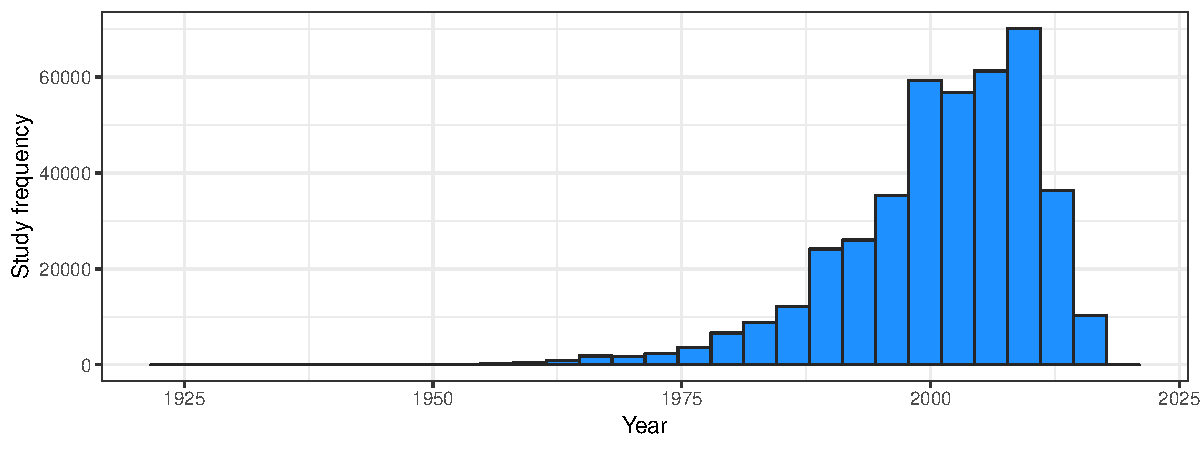
\includegraphics[width=\textwidth-3cm]{figure/ch02_figunnamed-chunk-8-1} 

}



\end{knitrout}
\caption{Frequencies of study publication years in the dataset. 44655 were excluded due to likely wrong indications.}
\label{study.years}
\end{figure}

Figure \ref{study.outcomes} provides the frequencies of outcome types of the comparisons. Note that the abundancy of mean differences and standardized mean differences can also give an impression of the proportion of continuous outcome comparisons vs. binary outcome comparisons in the dataset.

\begin{figure}
\begin{knitrout}
\definecolor{shadecolor}{rgb}{0.98, 0.98, 0.98}\color{fgcolor}

{\centering 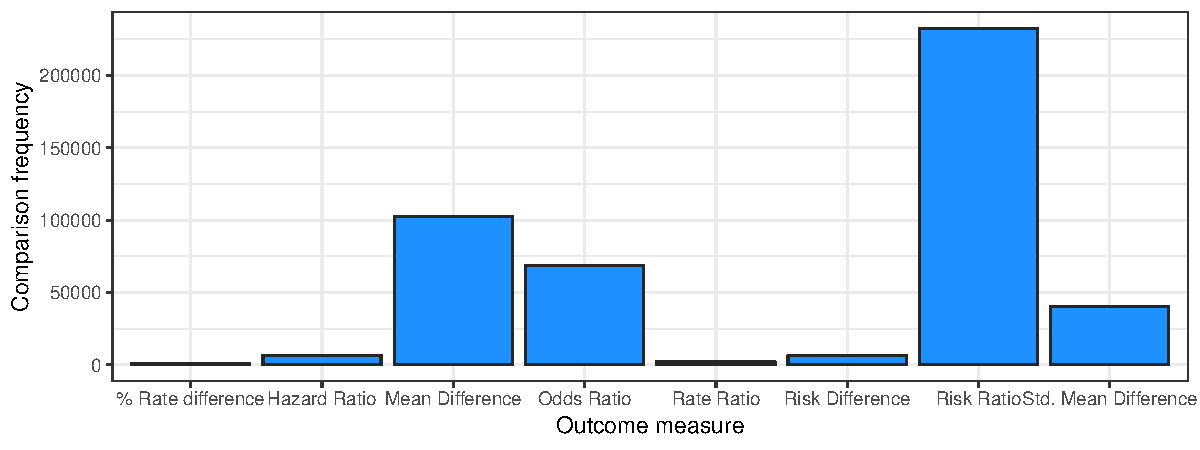
\includegraphics[width=\textwidth-3cm]{figure/ch02_figunnamed-chunk-9-1} 

}



\end{knitrout}
\caption{Frequencies of some outcome measures for the effects in the dataset. 5593 measures with other outcome measures are excluded.}
\label{study.outcomes}
\end{figure}

It is also possible to look at the properties of the reviews. One question could be how many studies or comparisons that a review comprises. The former is shown in Figure \ref{studies.per.review} and the latter in Figure \ref{comparisons.per.review}. It can be seen that while almost 400 reviews consist of one study only, there are more than 150 with equal or more than 30 distinct studies. A similar variance between reviews can also be observed when looking at the number of comparisons.

\begin{figure}
\begin{knitrout}
\definecolor{shadecolor}{rgb}{0.98, 0.98, 0.98}\color{fgcolor}

{\centering 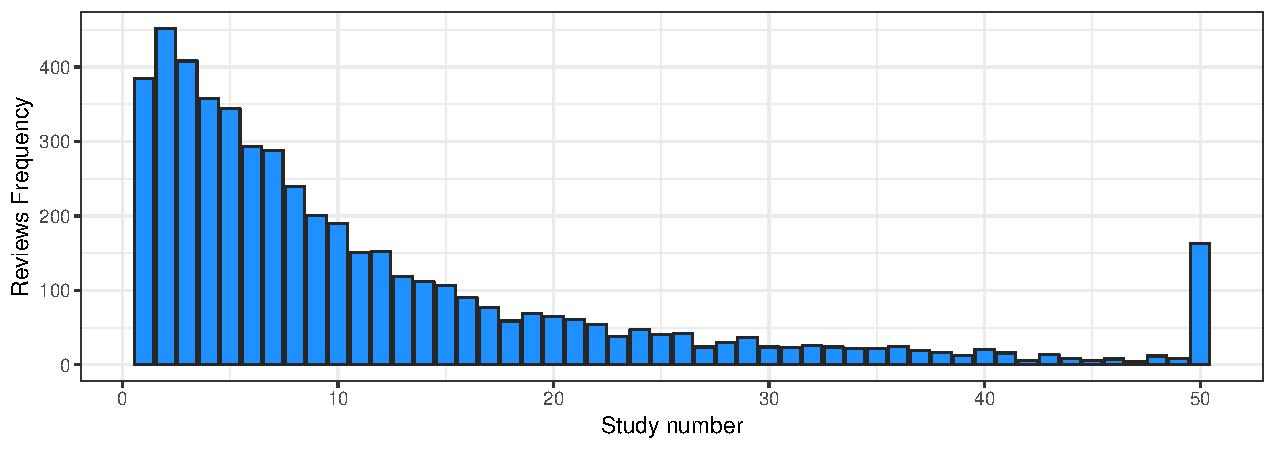
\includegraphics[width=\textwidth-3cm]{figure/ch02_figunnamed-chunk-10-1} 

}



\end{knitrout}
\caption{Empirical distribution of number of studies per review.}
\label{studies.per.review}
\end{figure}

\begin{figure}
\begin{knitrout}
\definecolor{shadecolor}{rgb}{0.98, 0.98, 0.98}\color{fgcolor}

{\centering 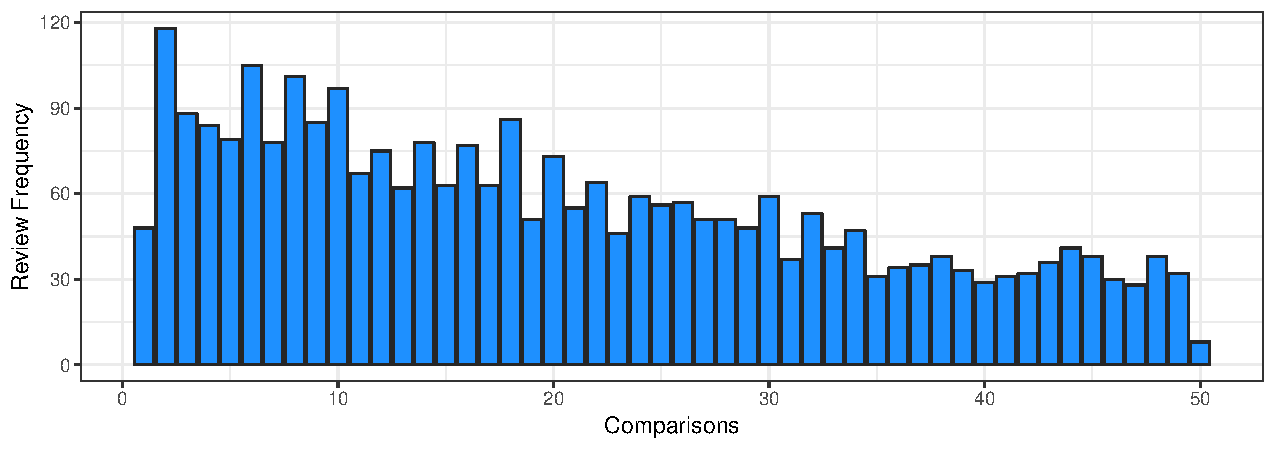
\includegraphics[width=\textwidth-3cm]{figure/ch02_figunnamed-chunk-11-1} 

}



\end{knitrout}
\caption{Empirical distribution of number of comparisons per review.}
\label{comparisons.per.review}
\end{figure}

A question not to be mistaken with the previous would be how many comparison \textit{types} there are per review. This gives an additional impression of the scope of a review. Analogously to the previous figures, the empirical distribution of comparison types is depicted in Figure \ref{subjects.per.review}.


\begin{figure}
\begin{knitrout}
\definecolor{shadecolor}{rgb}{0.98, 0.98, 0.98}\color{fgcolor}

{\centering 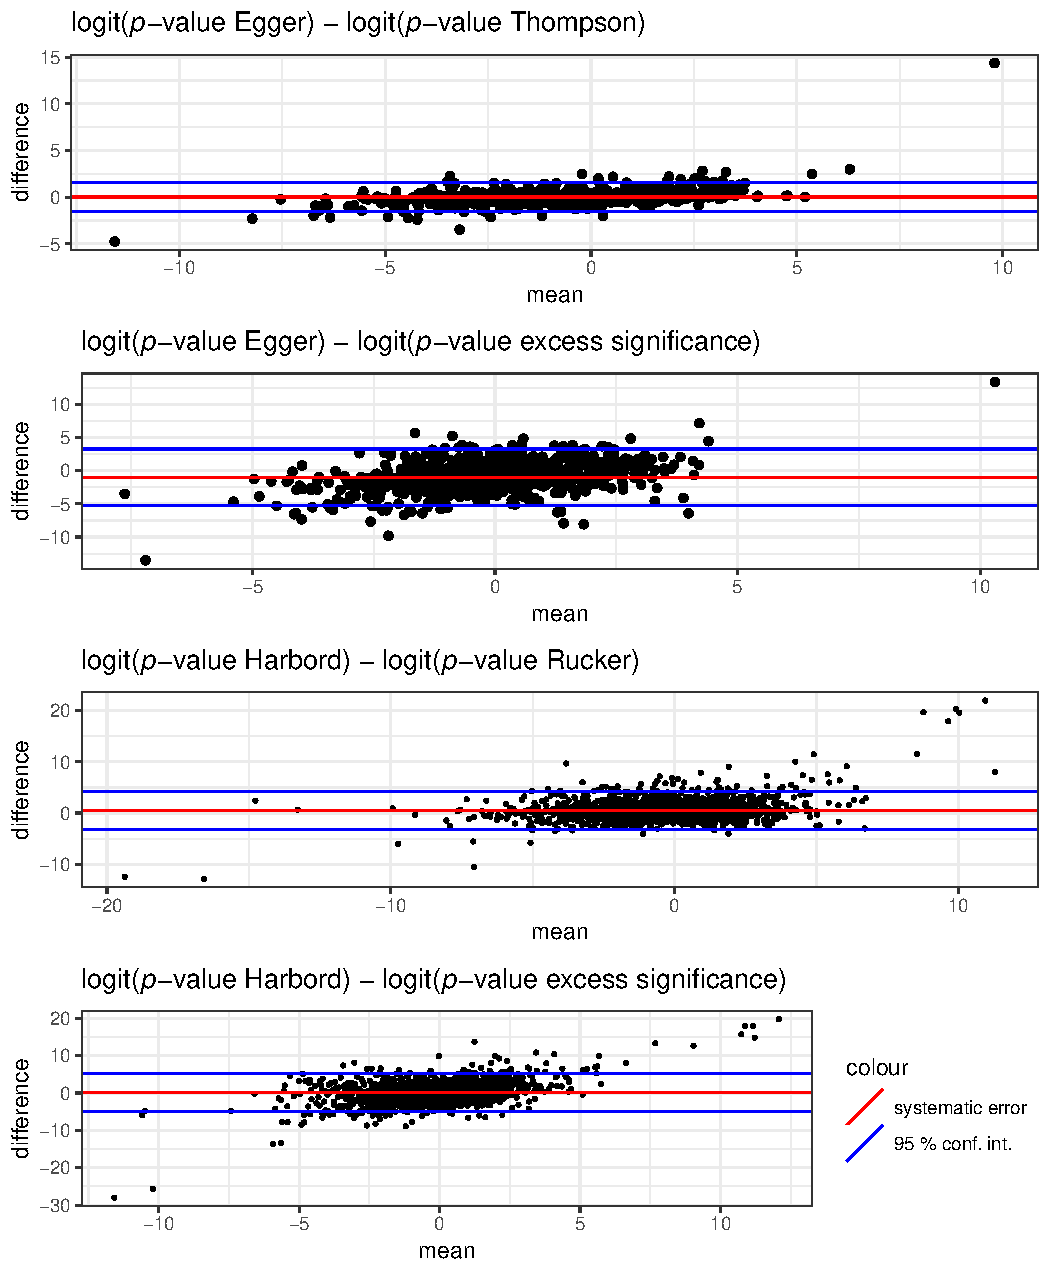
\includegraphics[width=\textwidth-3cm]{figure/ch02_figunnamed-chunk-12-1} 

}



\end{knitrout}
\caption{Empirical distribution of number of different research subjects per review.}
\label{subjects.per.review}
\end{figure}

% At the end, a main goal of the thesis is to analyze reviews with respect to reporting bias in meta analyses. 
For comparisons to be suitable for usage in meta-analysis, they have to be somewhat identical (same comparison type, outcome measure and possibly subgroup). For an analysis of reporting bias, again a certain number of studies is required in order for reporting bias to be detectable by the methods. One question would therefore be: How many groups of identical comparisons of a certain size are given in the dataset? This depends on which degree of similarity between comparisons is considered to be sufficient.

\vspace{0mm}
In Table \ref{repr.groups}, two different similarity criteria have been used. One is based on the same comparison type and outcome measure, the other includes additionally subgroup affiliation of comparisons, i.e. only comparisons in the same subgroups are considered to be similar enough.

\vspace{0mm}
Table \ref{repr.groups} shows the cumulative number of \textit{groups} of comparisons with equal or more than $n$ comparisons. Practically, this means that this number of meta analyses can be performed with each having at least $n$ comparisons.

% latex table generated in R 3.5.1 by xtable 1.8-3 package
% Thu Mar 21 11:15:10 2019
\begin{table}[ht]
\centering
\begingroup\footnotesize
\begin{tabular}{lll}
  \hline
n & Cumulative sum (without subgroups) & Cumulative sum (with subgroups) \\ 
  \hline
1 & 109177 & 186267 \\ 
  2 & 67685 & 83924 \\ 
  3 & 47786 & 52245 \\ 
  4 & 36155 & 36176 \\ 
  5 & 28077 & 26552 \\ 
  6 & 22689 & 20113 \\ 
  7 & 18536 & 15888 \\ 
  8 & 15466 & 12931 \\ 
  9 & 13000 & 10817 \\ 
  10 & 11001 & 9226 \\ 
  11 & 9356 & 7988 \\ 
  12 & 8052 & 7067 \\ 
  13 & 6984 & 6365 \\ 
  14 & 6041 & 5780 \\ 
  15 & 5325 & 5325 \\ 
   \hline
\end{tabular}
\endgroup
\caption{Cumulative number of groups with number of reproduction trials >= n} 
\label{repr.groups}
\end{table}





%%%%%%%%%%%%%%%%%%%%%%%%%%%%%%%%%%%%%%%%%%%%%%%%%%%%%%%%%%%%%%%%%%%%%%


% LaTeX file for Chapter 03









\chapter{Results}

One crucial assumption in meta analysis is that the availability and publication of studies does not depend on their effect. This is termed reporting bias in the scientific world. If reporting bias is present, the classical approaches to merge single study results in to an overall intervention effect may fail because the underlying studies are biased. There are tests that can be applied to find out if reporting bias is present in the meta analysis.

\vspace{0mm}
For continuous outcomes, three tests are available: Eggers (based on linear regression), Thompson and Sharp (weighted linear regression) and Begg and Mazumdar (rank based) test. The following three figures show the distribution of p-values of the corresponding tests. Note that only meta analyses with more than 10 comparisons have been included. 

\vspace{0mm}
Since each histogram of p-values has 20 bins, the content of the bin with the smallest p-values is equal to the number of meta-analyses whose reporting bias test reports a p-value < 0.05. The fraction of those analyses in which we would reject the null-hypothesis based on the 5 \% threshold can therefore be assessed by eye, and would be for example for Eggers test somewhat less than one third of all analyses. 

\begin{figure}
\begin{knitrout}
\definecolor{shadecolor}{rgb}{0.98, 0.98, 0.98}\color{fgcolor}

{\centering 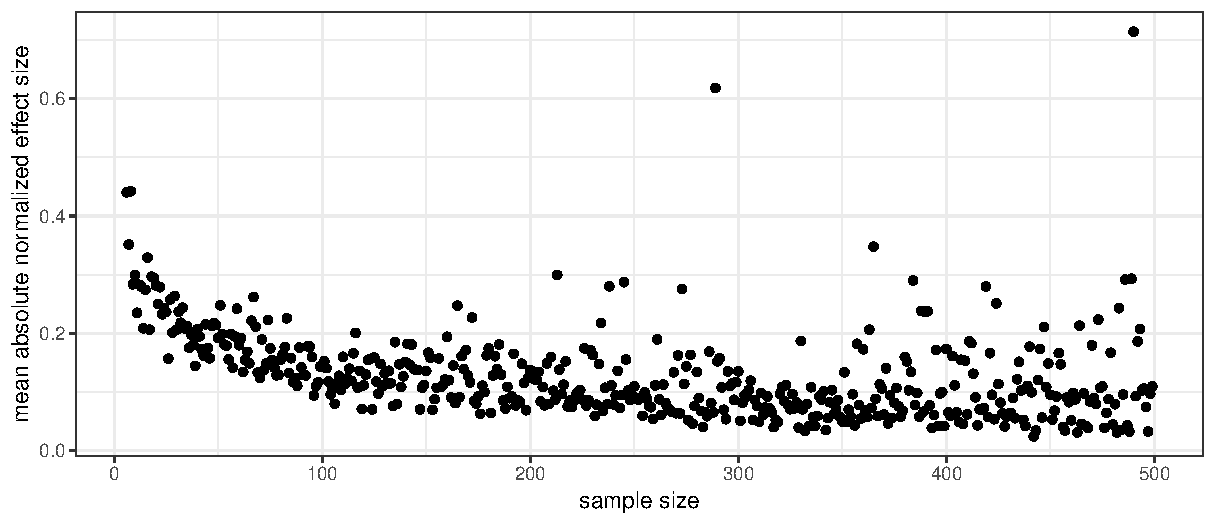
\includegraphics[width=\textwidth-3cm]{figure/ch02_figunnamed-chunk-17-1} 

}



\end{knitrout}
\caption{Histogram of p-values for Eggers reporting bias test (linear regression based) for continuous outcome meta analysis.}
\label{egger.cont}
\end{figure}


\begin{figure}
\begin{knitrout}
\definecolor{shadecolor}{rgb}{0.98, 0.98, 0.98}\color{fgcolor}

{\centering 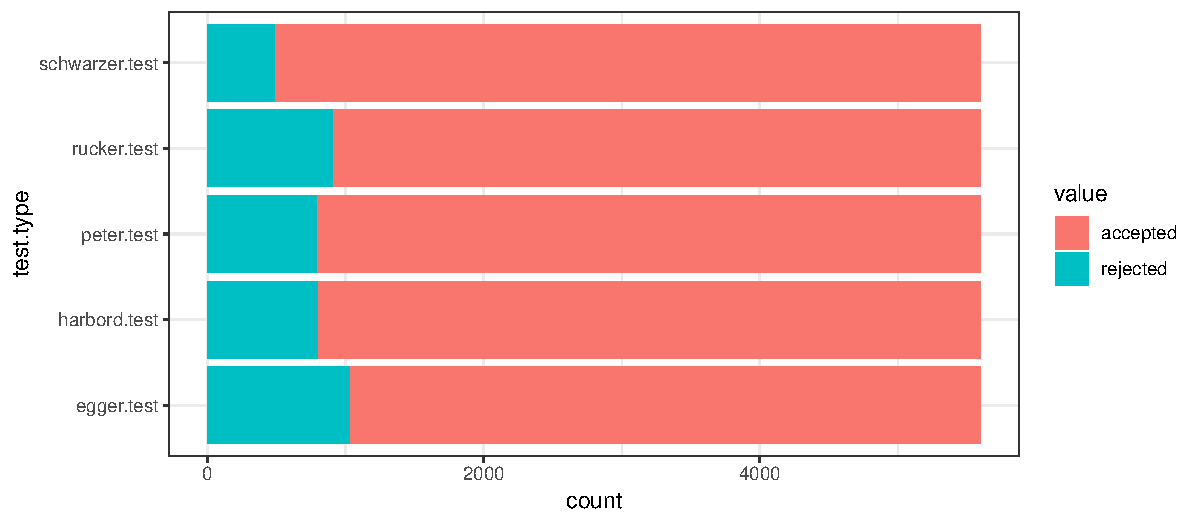
\includegraphics[width=\textwidth-3cm]{figure/ch02_figunnamed-chunk-18-1} 

}



\end{knitrout}
\caption{Histogram of p-values for Thompsom and Sharp reporting bias test (weighted linear regression based) for continuous outcome meta analysis.}
\label{thomson.cont}
\end{figure}

\begin{figure}
\begin{knitrout}
\definecolor{shadecolor}{rgb}{0.98, 0.98, 0.98}\color{fgcolor}

{\centering 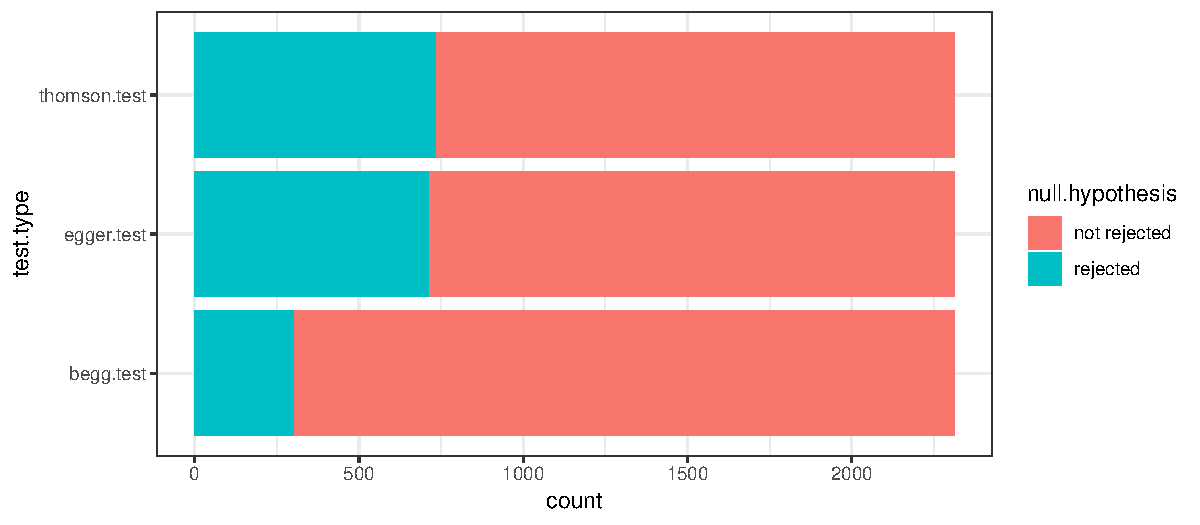
\includegraphics[width=\textwidth-3cm]{figure/ch02_figunnamed-chunk-19-1} 

}



\end{knitrout}
\caption{Histogram of p-values for Begg and Mazumdar reporting bias test (rank based) for continuous outcome meta analysis.}
\label{begg.cont}
\end{figure}


For binary outcomes, Peters and Harbords reporting bias test have been chosen. Also here, only meta-analyses with more than 10 comparisons are included.

\begin{figure}
\begin{knitrout}
\definecolor{shadecolor}{rgb}{0.98, 0.98, 0.98}\color{fgcolor}

{\centering 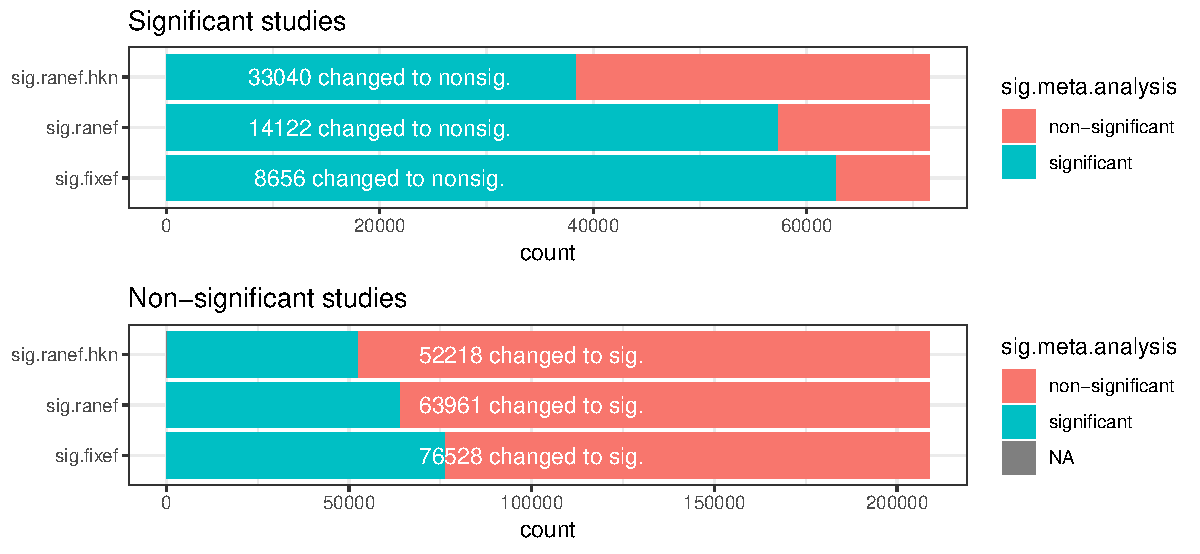
\includegraphics[width=\textwidth-3cm]{figure/ch02_figunnamed-chunk-20-1} 

}



\end{knitrout}
\caption{Histogram of p-values for Peters reporting bias test (rank based) for continuous outcome meta analysis.}
\label{peters.bin}
\end{figure}


\begin{figure}
\begin{knitrout}
\definecolor{shadecolor}{rgb}{0.98, 0.98, 0.98}\color{fgcolor}

{\centering 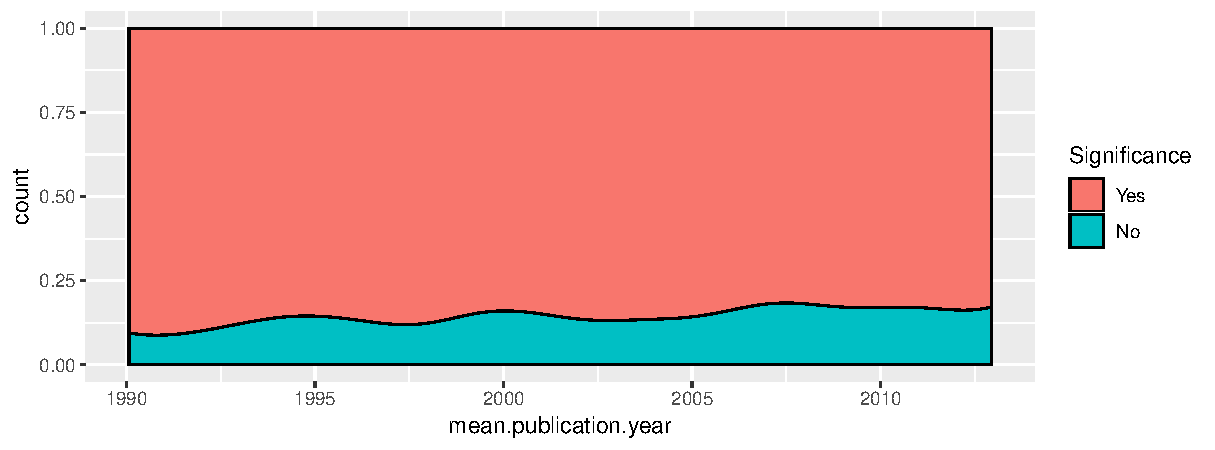
\includegraphics[width=\textwidth-3cm]{figure/ch02_figunnamed-chunk-21-1} 

}



\end{knitrout}
\caption{Histogram of p-values for Harbord reporting bias test (rank based) for continuous outcome meta analysis.}
\label{harbord.bin}
\end{figure}




Another less conventional way to look for publication bias is to see how many studies are ``reflected'' by the trim and fill method. As a first impression, a histogram with the fraction of trimmed of all comparisons is shown in figure \ref{trimfill.cont}. 

\begin{figure}
\begin{knitrout}
\definecolor{shadecolor}{rgb}{0.98, 0.98, 0.98}\color{fgcolor}

{\centering 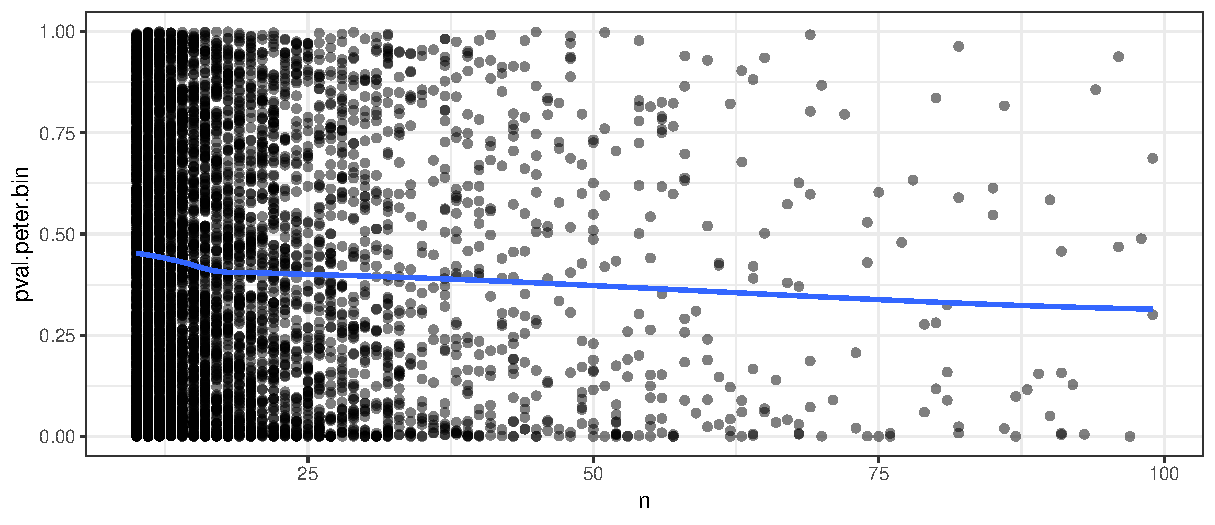
\includegraphics[width=\textwidth-3cm]{figure/ch02_figunnamed-chunk-22-1} 

}



\end{knitrout}
\caption{Histogram of fractions of trimmed comparisons from meta analyses with continuous outcomes.}
\label{trimfill.cont}
\end{figure}

The mean fraction of trimmed comparisons for continuous outcomes is 0.22 and the median 0.2.

The same is repeated for binary outcomes in figure \ref{trimfill.bin}. 
\begin{figure}
\begin{knitrout}
\definecolor{shadecolor}{rgb}{0.98, 0.98, 0.98}\color{fgcolor}

{\centering 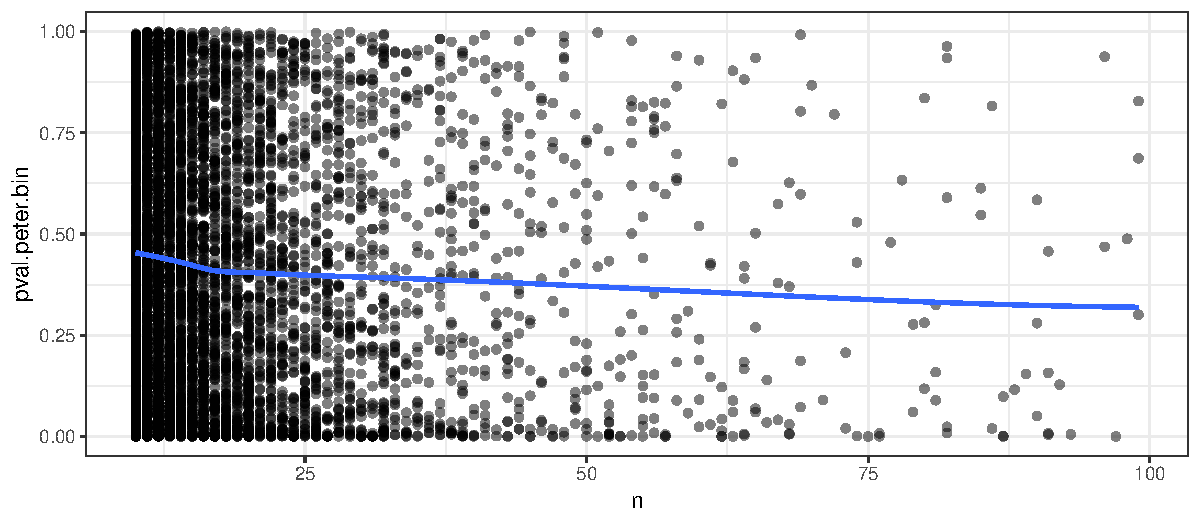
\includegraphics[width=\textwidth-3cm]{figure/ch02_figunnamed-chunk-23-1} 

}



\end{knitrout}
\caption{Histogram of fractions of trimmed comparisons from meta analyses with binary outcomes.}
\label{trimfill.bin}
\end{figure}

The mean fraction of trimmed comparisons for binary outcomes is 0.19 and the median 0.17.


%%%%%%%%%%%%%%%%%%%%%%%%%%%%%%%%%%%%%%%%%%%%%%%%%%%%%%%%%%%%%%%%%%%%%%


% LaTeX file for Chapter 04


\chapter{Discussion and Outlook}


%%%%%%%%%%%%%%%%%%%%%%%%%%%%%%%%%%%%%%%%%%%%%%%%%%%%%%%%%%%%%%%%%%%%%%


% LaTeX file for Chapter 05


\chapter{Conclusions}

%%%%%%%%%%%%%%%%%%%%%%%%%%%%%%%%%%%%%%%%%%%%%%%%%%%%%%%%%%%%%%%%%%%%%%

\appendix

% LaTeX file for Chapter 01



\chapter{Appendix}

Maybe some R code here, probably a \rr{sessionInfo()}




\cleardoublepage
\phantomsection
\addtocontents{toc}{\protect \vspace*{10mm}}
\addcontentsline{toc}{chapter}{\bfseries Bibliography}


\bibliographystyle{mywiley} 
\bibliography{biblio}

\cleardoublepage

\end{document}

